The preceding results examined various aspects of model fit, and Sections~\ref{res:post_contour} and~\ref{res:marginal} highlight an especially intriguing finding. Specifically, the marginal posterior of $\lambda$ is unaffected by the prior choice on $A$, as long as the support condition $A \geq y_{\max}$ is satisfied. This separability is unusual in multi-parameter Bayesian survival models, where parameters typically remain entangled and sensitive to prior assumptions. Here, however, the inference for the event-rate parameter $\lambda$ remains robust, while $A$ serves only to capture the structural features of the censoring mechanism. In practical terms, this means $\lambda$ can always be stably estimated, while $A$ captures censoring structure without distorting inference on the underlying hazard rate. 

While this theoretical robustness is reassuring, posterior predictive checks simultaneously reveal practical shortcomings of the exponential baseline. As shown in Section~\ref{res: model checking}, the constant hazard assumption fails to capture the empirical feature of the data, namely a “steep early rise followed by a gradual decline.” This results in a systematic underestimation of event occurrences in the mid-range. To address this mismatch, it is natural to consider alternative distributions, especially those that allow hazards to vary over time and possibly take non-monotonic forms.

Before moving to such flexible specifications, however, it is natural to first reflect on a monotone alternative: the Weibull model. Although Weibull introduces time dependence, its single shape parameter limits flexibility, making it difficult to accommodate both the sharp early risk and the smoother decline in later periods (as illustrated more clearly in the supplementary figures, such an adjustment does not lead to noticeable improvement). Hence, models with monotone hazards are not suitable for this dataset. This reflection points toward a more promising direction: models that allow non-monotone and locally curved baseline hazards.

A natural candidate is the piecewise-constant hazard (PWE) model. Dividing time into intervals permits the hazard to vary flexibly across segments, thereby directly capturing the “early steep, later flat” turnover pattern observed in the data. Here, I illustrate this approach with a simplified version using six segments, while keeping the observation window fixed at $A=179$ for comparability with the exponential model. The posterior predictive results show that the ECDF of event times improves markedly, indicating that such models align more closely with the structure of the data.
\begin{figure}[H]
    \centering
    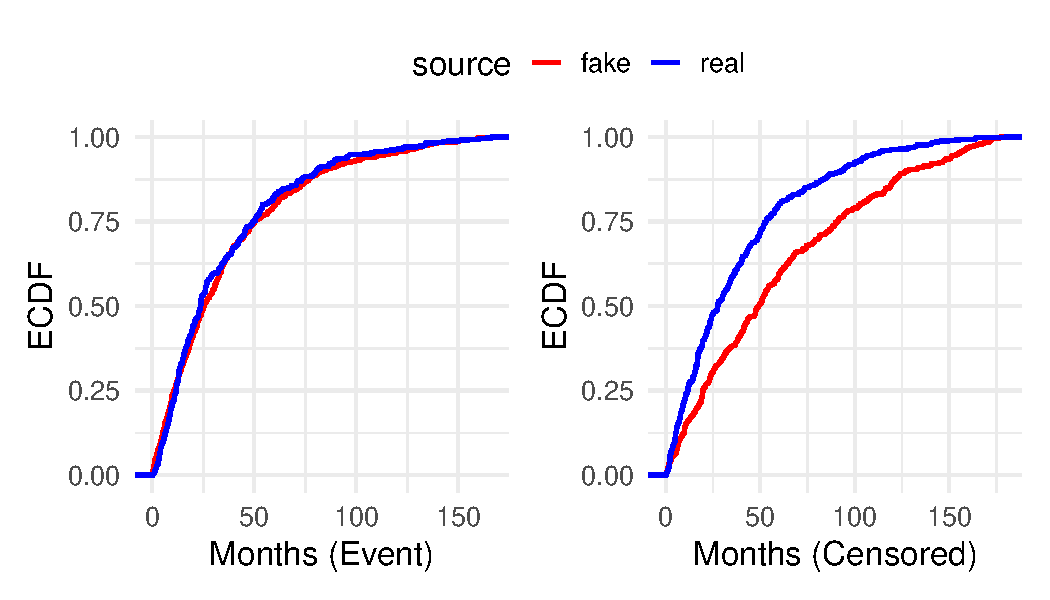
\includegraphics[height=6cm, width=0.75\textwidth]{images/piece6_ecdf_comparison.pdf}
    \caption{{\small Posterior predictive ECDFs of event times (left) and censored durations (right) under a six-segment piecewise-constant hazard model (cuts at 40, 75, 105, 120, 160, 200), with $A=179$ fixed for comparability.}}
    \label{fig:ppc_map}
\end{figure}
However, this exercise also reveals another issue that even under the PWE framework, the fit for censoring remains problematic. The observed censoring ECDF lies systematically above the simulated one. This discrepancy does not arise from the event process but rather from the censoring mechanism. In the current PPC setting, we assume uniform entry over $[0, A]$, such that censoring is entirely administrative. In reality, however, recruitment may not be uniform—for instance, if the company recruits heavily in later periods, this would generate more early censoring. This explains the “excess censoring” observed in the real data and suggests that future work should incorporate entry mechanisms informed by the company’s operational context.

Finally, it is important to note that modeling choices depend on research objectives. If the aim is to characterize overall turnover trends, improving the baseline hazard and censoring mechanism may already provide useful conclusions. But if the goal is to predict turnover risk at the individual level, covariates must be incorporated to account for heterogeneity across employees.

